\documentclass[mathserif]{beamer}
%\documentclass[mathserif,handout]{beamer}
%\documentclass[dvips]{beamer}
\definecolor{Beige}{rgb}{0.96,0.96,0.86}
\definecolor{Yellow}{rgb}{1.,0.84,0.8}
\definecolor{Gold}{rgb}{1.,0.84,0.}
\definecolor{RedA}{hsb}{0.9,0.3,0.7}
\definecolor{RedB}{hsb}{0.9,0.3,1}
\definecolor{LightGray}{gray}{0.85}
\definecolor{Blue}{rgb}{0.,0.,1.}
\definecolor{Pink}{rgb}{0.9,0.75,0.8}
\definecolor{DarkGreen}{rgb}{1.0,1.0,1.0}
\definecolor{DarkBlue}{rgb}{0.,0.5,1.0}
%\definecolor{Pink}{rgb}{1.,0.75,0.8}
\definecolor{LightCyan}{rgb}{0.88,1.,1.}
%\definecolor{LightYellow}{rgb}{0.95,1.0,0.8}
\definecolor{red1}{rgb}{0.95,0.,0.}
%\definecolor{mycol1}{rgb}{0.9,0.2,0.9}
%\definecolor{mycol1}{rgb}{0.5,0.8,0.4}
\definecolor{mycol1}{rgb}{0.5,0.6,0.8}
\definecolor{mycol2}{rgb}{0.6,0.8,0.6}
\definecolor{LightYellow}{rgb}{0.95,1.0,0.8}

\mode<presentation>
{
%\usepackage{beamerthemeCambridgeUS, fancybox}
\usepackage{fancybox}
\usepackage{graphicx}
\usepackage{subfigure}
\usepackage[english]{babel}
\usepackage{multirow}
\usepackage{verbatim}
\usepackage{verbatim,epsfig,graphics,amssymb,amsmath,subfigure}
\usepackage{helvet}
\usepackage{graphicx}
\usepackage{wrapfig}
\setbeamercovered{transparent}
}
%\usepackage[T1]{fontenc}
%\usepackage[adobe-utopia]{mathdesign}
%\usepackage{fouriernc}
\usepackage[bitstream-charter]{mathdesign}
\usepackage[T1]{fontenc}



\usefonttheme{serif}

\usetheme{Boadilla} 

\setbeamertemplate{navigation symbols}{}
\setbeamersize{text margin left=3mm, text margin right=3mm}
\newcommand{\B}[1]{\boldsymbol{#1}}
\usepackage[all]{xy}
\usepackage[utf8]{inputenc}
%\usepackage{pdfpages}


\title[Seed-grant proposal]
{Multimodal classification of birds\\
\small{Seed-grant proposal}}

%\author[Paddy]{R. Padmanabhan (Paddy)}
\author[ADP]{Arnav Bhavsar\\
		Dileep A. D.\\
		Padmanabhan Rajan
}

\institute[IIT Mandi] {
Multimedia Analytics and Systems Lab\\
School of Computing and Electrical Engineering\\
%Indian Institute of Technology Mandi \\
\includegraphics[width=4cm,height=2cm]{figures/mas_logo.pdf}
\includegraphics[width=3cm,height=2cm]{figures/iitmandi-logo.pdf}
}
%\date[November 11th, 2009]
{}

%%%%%%%%%%%%%%%%%%%%%%%%%%%%%%%%%%%%%%%%%%%%%%%%%%%%%%%%%%%%%%%%%%%%%%%%%%%%%%%%%%%%%%%%%%%%%
\begin{document}
\normalfont

%%%%%%%%%%%%%%%%%%%%%%%%%%%%%%%%%%%%%%%%%%%%%%%%%%%%%%%%%%%%%%%%%%%%%%%%%%%%%%%%
\begin{frame}
        \titlepage
\end{frame}

%\logo{\includegraphics[height=0.8cm]{figures/iitmandi-logo.pdf}\vspace{220pt}}
\logo{\includegraphics[height=0.8cm]{figures/mas_logo.pdf}\vspace{220pt}}


\begin{frame}
\frametitle{Overview}
\begin{wrapfigure}{r}{0.5\textwidth}
\centering
%  \begin{center}
    \includegraphics[width=0.48\textwidth]{figures/parakeet.jpg}
%  \end{center}
  \caption{\small{Slaty-headed parakeet. Pic by PPJ.}}
\end{wrapfigure}
The objective\\
The acoustics\\
The image/video\\
This machine learning\\
The budget and other details\\
\end{frame}

\begin{frame}
\frametitle{The objective}
\begin{itemize}
\item<2-> Develop algorithms for automatic analysis of avain biodiversity
\item<3-> Combine information from acoustic and visual data streams
\item<4-> Sensors: microphones, cameras
\item<5-> Apply signal processing and machine-learning techniques to collected
data
\item<6-> Tasks: Species identification, species detection
\end{itemize}
\end{frame}

\begin{frame}
\frametitle{The motivation}
\begin{itemize}
\item<2-> Birds provide crucial ecosystem services: pollination, seed dispersal,
insectivory
\item<3-> Avian diversity: good indicator of ecosystem health in a local area
\item<4-> Automatic and semi-automatic sensing devices can be utilised
\item<5-> Large volume of data captured by these devices
\item<6-> Algorithms to analyse this data would be useful to ecologists
\end{itemize}
\end{frame}

\begin{frame}
\frametitle{The challenges}
\begin{itemize}
\item<2-> 
\item<3-> Avian diversity: good indicator of ecosystem health in a local area
\item<4-> Automatic and semi-automatic sensing devices can be utilised
\item<5-> Large volume of data captured by these devices
\item<6-> Algorithms to analyse this data would be useful to ecologists
\end{itemize}
\end{frame}




\begin{frame}
\frametitle{Speech activity detection (SAD)}
\begin{figure}[t12]
\centering
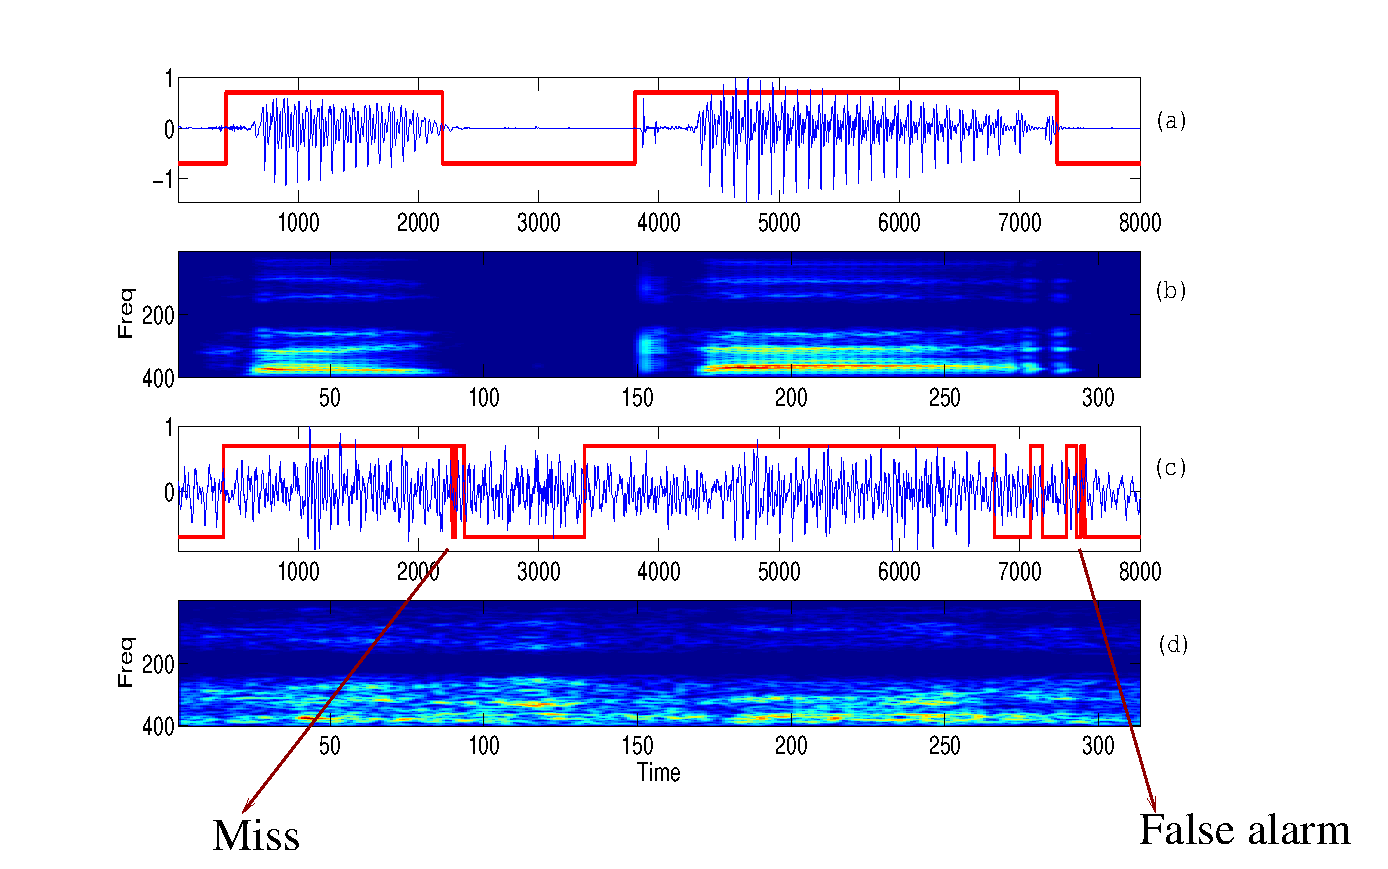
\includegraphics[width=10cm,height=6cm]{figures/vad_miss_fa.eps}
\end{figure}
\begin{itemize}
	\item SAD is challenging in noisy conditions
\end{itemize}
\end{frame}



\begin{frame}
\frametitle{}
\Large{Thank you for your attention.}
\end{frame}


\end{document}

